% Guidance: maximum 3 pages for this section. Since we have 6-7 sub-sections, each should be 1/2 page maximum.

We anticipate that distributed sites will continue to provide the bulk of resources used for data processing, simulations and analysis in the HL-LHC era. This infrastructure is expected to be provided via WLCG mechanisms based on bilateral agreements (MoU) between WLCG and contributing funding agencies that cover the entire duration of the LHC program, including HL-LHC. ATLAS has a sophisticated distributed computing system (ADC) that optimally makes available hundreds of clusters and associated storage at distributed WLCG sites. ADC provides a fully integrated system for all workflows and for all users. The automated tools developed by ADC include ProdSys, PanDA, Rucio, SSB, HammerCloud, and others. These tools will continue to be upgraded and evolve as needed. Many of the upgrade plans require tighter future integration among tools to improve efficiency in the more complex environment of the HL-LHC. Below we provide a few examples of long range R\&D plans which are needed to transition to the new challenges at the HL-LHC. The metrics used to evaluate progress with the R\&D projects will include: scalability for HL-LHC, improved efficiency in resource usage (CPU, storage and network), and improved operational efficiency. We anticipate all the new R\&D projects described here will require additional effort or redirection of effort.

\subsection{Evolution of WLCG}
\label{sec:wlcg}

WLCG strives to accommodate many scientific endeavours in future, and already now DUNE~\cite{DUNE2018} and Belle-II~\cite{Belle-II} have joined the infrastructure. More projects are expected to join soon, most notably, those that take part in the European ESCAPE~\cite{EU-ESCAPE} cluster of ESFRI activities. The overarching challenge for all these projects is distributed data handling, therefore WLCG focuses on R\&D in the areas of Data Organisation, Management and Access (DOMA), which is expected to have impact in terms of the data infrastructure and services. In particular, the Data Lake approach (see Section~\ref{sec:lakes}), under development and evaluation by current R\&D projects (DOMA, ESCAPE, IRIS-HEP, and others), will have implications on data placement, delivery and caching, which will need to be properly accommodated by ATLAS tools and services. Specifically, multi-level caching via Xcache, third-party transfer implementation without GridFTP, token-based authentication and quality of service criteria will have to be implemented in ATLAS distributed computing tools. 

Earlier (in Figure~\ref{fig:2018Res}) we showed the resource challenges facing the HL-LHC. Many R\&D activities have already started to address the CPU challenge -- we expect that the CPU deficit will be substantially reduced through these efforts described in other sections. However, the storage and network challenges are formidable, which will be partly addressed through the WLCG DOMA project. Later in this section we describe a few additional R\&D projects to manage the storage shortfall, like Data Carousel and iDDS, which are specific to ATLAS.

%how do we make it quantitative?

\subsection{PanDA and ProdSys}

PanDA is the ATLAS workload management system used to execute all scientific workflows for all users on widely distributed heterogeneous resources. It is tightly integrated with the ATLAS distributed data management system, Rucio. For the HL-LHC, the PanDA development team has started multiple R\&D efforts. The Data Carousel project, the ProdSys system, HPC and cloud orchestration, and the intelligent Data Delivery System are prominent examples described separately. In addition, the PanDA team is working on global shares and unified queues, edge services through Harvester, MPI services, event service, SciTokens authentication, active network management, operational intelligence, anomaly detection, and machine learning techniques. We anticipate that one to two FTE effort will be needed for these R\&D topics for the next three years. The overall goal is to meet the HL-LHC scale and resource capacity challenges without sacrificing the flexible ADC system.

ProdSys is the primary interface between users and PanDA, providing a task management interface. New workflows are regularly developed in ProdSys. Monitoring systems are evolved to meet new requirements. The most disruptive challenge facing ProdSys is the growing importance of machine learning techniques, especially for distributed training. New schemas are being developed for non-traditional HEP use cases that are not collision event based. As new analysis models emerge for HL-LHC, we expect major additions to ProdSys capabilities. R\&D efforts in ProdSys for the HL-LHC will be primarily focused on supporting non-traditional workflows. We estimate this effort to require half FTE over three years.

\subsection{Rucio}

Rucio is an open-source software framework that provides scientific
collaborations with the functionality to organize, manage, monitor, and
access their distributed data at scale. The system manages more than 500
petabytes spread on 130 data centres with 600 storage locations, with
daily data access of over 12PB, as well as over 2PB of data transfers,
deletion, and recovery. The success of Rucio in the ATLAS experiment has
led to it being adopted as the data management system by the CMS,
XENON-1T, and AMS experiment and it is under evaluation by several other
established and upcoming experiments such as Belle 2, DUNE, LIGO/VIRGO,
and SKA.

Future developments, specifically aimed at the HL-LHC era, aim to
further improve the scalability of the system, to ensure that the system
scales to the requirements of HL-LHC data rates. These developments are
already starting now and especially target the improvement of the
deletion and transfer evaluation components of the system. Further
developments are planned to evolve the metadata component to support
future workflows as well as to introduce the functionality of storage
Quality of Service (QoS) to the system. Although Rucio already supports
numerous database back-ends, such as Oracle, MySQL, and PostgreSQL,
special emphasis is being made to ensure that the database interactions
scale for Non-Oracle databases. Additionally, as more experiments and
communities at similar data rates as the HL-LHC will come online in the
next years, another development will be orchestration of dataflows
across multi-experiment Rucio installations, as well as direct
integration with the network layer for dynamic provisioning of bandwidth.

% Can Rucio team provide estimate of how much additional effort is needed for R&D?

\subsection{Data Carousel and iDDS}
The cost of disk storage will be prohibitive for our current workflow patterns at HL-LHC volumes. We must therefore make better use of cheaper media with lower QoS - today this means magnetic tape, but the method does not exclude others, for example spun-down hard disk.
The Data Carousel orchestrates data processing across workload
management, data management, and storage services with the bulk data
resident on offline storage. The processing is executed by staging and
promptly processing a sliding window of inputs from faster buffer storage,
such that only a small percentage of input data are available at any time. With this project we aim to demonstrate that this is the natural way to
dramatically reduce our storage cost. The first phase of the project was
started in the Autumn of 2018 and was related to I/O tests of the sites archiving
systems. Phase II requires a tight integration of the workload and data management systems and will be used already in Run3 for processing RAW data. At HL-LHC we will need to go further and store reconstructed data principally on tape, to be processed using the Data Carousel. This will require further developments such as 
file level staging-job orchestration through intelligent Data Delivery Service (iDDS). The iDDS system in PanDA is being developed to provide streaming services for data delivery for a wide range of workflows. Data Carousel is an important and first proof of concept demonstration of iDDS for ATLAS.

%\subsection{Streaming Data Services}
%In order to support new analysis methods \cite{streaming} we will need to produce custom data formats in quasi-realtime and stream to user analysis facilities. ServiceX will produce data in a columnar format suitable for highly parallel processing. iDDS would enable a user feedback loop into multi-step analysis chain.
% not sure I understand this, but both are referenced from the analysis section

%\subsection{Machine Intelligence for Workflow Management}
%KD


\subsection{Infrastructure}

\subsubsection{Facilities and operations}

%IMPORTANT: stress the need for "own" custom facilities, as opposed to generic HPC ones. Do we have to speculate on evolution of facilities? Containerized Data Centres? Microservices? DevOps?
%Tier 1 vs Tier 2 difference is gone (except for tape and 2nd copy of data)
%evolve towards facilities based on capability rather than Tier label

While the rigid hierarchical distinction between Tier 1 and Tier 2 sites already disappeared in ATLAS during Runs 1 and 2, these sites will continue to be the backbone of the computing infrastructure for ATLAS at the HL-LHC. Tier 1 sites are expected to continue providing custodial service for primary data through tape storage. A more flexible classification of sites based on capabilities is emerging. Sites will be classified based on infrastructure and workload capabilities irrespective of their Tier label. HPC, Cloud and other opportunistic resources are expected to extend the capabilities of ATLAS managed Tier 1 and Tier 2 sites, but not replace their custodial roles or provide the wide array of time critical processing and storage services.

\subsubsection{Analysis Facilities}
During Runs 1 and 2, WLCG Tier 1 and 2 sites provided distributed processing capability for ATLAS analysis users, at the scale of a million analysis jobs executed per day. However, these facilities are not well suited for the final interactive stages of user analysis, for example visualizations, plot generation, re-weighting, systematic studies, limit testing, etc. Local sites (often called Tier 3 sites), funded and managed outside the WLCG framework, often provided the necessary resources for end-user analysis. Many of these sites are connected through ADC tools like PanDA and Rucio. The future of these analysis facilities depends on the success of new analysis tools and analysis models. R\&D work is needed to determine the size, scale and cost of analysis facilities. Metrics of reduced cost, increased efficiency and scalability need to be demonstrated. This R\&D work is dependent on the analysis tools R\&D described earlier in the document, and will require additional effort of a few FTE to evolve the future analysis facilities.


\subsubsection{Data Lakes}
\label{sec:lakes}
A possible future direction for WLCG storage is to extend the concentration of disk resources at fewer and larger, possibly federated, sites. Smaller cache-like storage would serve the more widely 
distributed computing resources. The reasoning is that the provisioning and operation of robust storage requires significantly more manpower, than needed for a compute cluster with a cache of secondary replicas. In principle, distributed operations are simplified in this scenario, although separation of storage and computing raised their own reliability and operational challenges in the past. Results from a WLCG survey suggest the manpower requirement is perhaps not a driving factor for the typical Tier2. Also local and regional funding tends to work against concentration of resources. Nevertheless, some sites or funding agencies have already chosen to connect computing facilities to remote storage through cache layer. We need to prepare for a significant fraction of remote accesses.

\subsubsection{Network}
\label{sec:network} 
The exponential growth of essentially free research network bandwidth has thus far enabled an abstraction of the ATLAS data transfer activities from the underlying network. The major developments likely to affect ATLAS are packet marking, new cost models and programmable WAN links.  

Packets traveling on dedicated WLCG sections of the network will be marked by the application, in order to attribute the activity to a particular Virtual Organization (VO). This capability is especially important because it is not always clear what the impact to wide-area networking is when making changes to our complex, global infrastructure. Being able to identify owners and types of traffic flows anywhere in the network makes it possible to identify the root cause for significant changes in network traffic.  Another consideration is that the cost for a particular bandwidth, for example transatlantic, may become more direct, rather than hidden in general research network budgets. In addition, usage of commercial cloud storage egress incurs very clear costs for the experiment.  Programmable WAN links offer the potential to be able to boost bandwidth between sites on demand.

Rucio has a matrix of connectivity and bandwidth between sites, with information taken from the File Transfer Service (FTS) and manual input. This will be augmented with information about cost and potential programmable links. PanDA can use this to influence job placement, but will need improvements to optimize for speed or cost.

Much of this work is being discussed in twice yearly LHCONE/LHCOPN meetings and has been reported on by the HEPiX Network Function Virtualization working group in their phase I report\cite{hepix_nfv_working_group_2019_3565563}.  

It is important to note that ATLAS will need to work more closely with both the national research and education networks and the various networking research efforts to effectively prepare for the HL-LHC era. In early 2020 there are efforts underway to create a networking technical working group to discuss, document and prototype capabilities identified as being important for the LHC experiments.  ATLAS also needs to be ready to take advantage of international scale network testbeds capable of providing a geographical footprint, advanced services and capacities relevant for the HL-LHC.  Testbeds like that will be critical for testing network capabilities and services to evaluate their impact for ATLAS in the context of HL-LHC. 

%Need to cut down HPC section below to fit 1/3rd to 1/2 page. Seems cut already.

\subsubsection{Non-dedicated High Performance Computing resources}
\label{sec:hpc}

Due to the large amount of data used by ATLAS, currently about half an Exabyte for all data products and growing, and custom developed software applications specific to ATLAS, it is considered optimal for ATLAS to use dedicated resources at Tier 1 and Tier 2 sites, starting with specially configured networks (Sec.~\ref{sec:network}), storage facilities (Sec.~\ref{sec:lakes}) and computing resources. These sites are mostly large clusters similar to those at CERN. The vast majority of resources pledged by contributing countries and those used for Runs 1 and 2 at the LHC, are thus hardware built for ATLAS and other LHC experiments. Without these dedicated resources, some computing workflows will need to be rationed, thereby reducing the scope of physics results produced by ATLAS. It is anticipated that the current resource deployment will continue in the future: most national particle physics communities will retain the ability to build and maintain dedicated IT infrastructures for ATLAS needs.

Historically, some significant resources were pledged to ATLAS through allocation or dedicated partitions at generic public High-Performance Computing facilities. One notable example is the NDGF Tier1~\cite{ndgf} where all computational power is provided via national research data centers shared with other scientists. It is anticipated that in future more resource providers will use this model, and a larger part of the pledged resources will come through non-dedicated shared facilities. While they will still be a part of the WLCG infrastructure, ATLAS will have to cope with the necessity to adapt to such resources in terms of e.g. processor architectures, operating systems, file systems, quotas etc.

% Bibliography is needed for Leadership machines and backfill success stories
At the same time, very large HPC facilities, for example the Leadership Class Facilities~\cite{leadership} funded by the U.S. Department of Energy, are known to have large idling capacity due to the nature of their main workloads. Such facilities are willing to accept serial payloads from ATLAS as a back-fill~\cite{backfill}. With an increased investment in Europe and worldwide into exascale computing it is safe to assume that more such opportunities will appear in future, and a significant computing capacity will become available opportunistically, i.e., outside of the service levels as defined in the WLCG MoU~\cite{wlcg-mou} and not subject to WLCG policies and operational procedures in general. In this case ATLAS will have to cope not only with local architecture peculiarities and policies, but also with the fact that such facilities are not a part of the WLCG operations. This will limit the workloads that we can run, and part of the preparations for HL-LHC will be R\&D to run more challenging workloads, such as data-intensive or those requiring extensive database access at HPC sites. This can only work if HEP requirements are taken into account in both the design and policies of the HPC facilities. We estimate one FTE additional effort for HPC R\&D.


%\begin{figure}[ht!]
%\caption{Evolution of the share of accelerators and co-processors in Top500 HPC systems %(source: top500.com). A trend towards an increasing share of such can be seen.
%\label{fig:top500-gpu}}
%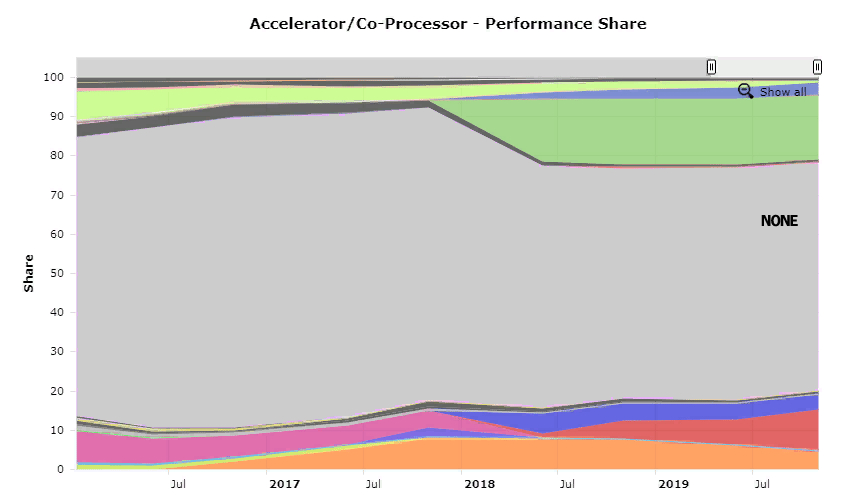
\includegraphics[width=12cm]{figures/Top500-coprocessors.png}
%\end{figure}

%Challenges:
%\begin{itemize}
%    \item Heterogeneous architectures are likely to become dominant, implying that less capacity will be available through conventional CPUs. % see Fig.~\ref{fig:top500-gpu}.
%    \item Opportunistic resources have no formal Service Level Agreements consistent with the rest of the infrastructure.
%    \item Local to HPC policies may be inconsistent with ATLAS ones, such as e.g. limited access to users outside the host country.
%\end{itemize}